\documentclass[11pt,a4paper]{article}
\usepackage[margin=25mm]{geometry}
\usepackage[T1]{fontenc}
\usepackage{lmodern,microtype}
\usepackage{amsmath,amssymb,mathtools,bm}
\usepackage{graphicx,booktabs,array}
\usepackage{subcaption}
\usepackage{placeins}
\usepackage[numbers,sort&compress]{natbib}
\usepackage{xcolor}
\usepackage[unicode,colorlinks=true,linkcolor=blue!50!black,citecolor=blue!50!black,urlcolor=blue!50!black]{hyperref}
\usepackage{url}
\hypersetup{pdftitle={MAcNLOPS from ordinary MC@NLO events: signed residuals, shower support and mass conventions},pdfsubject={Common-source signed-residual implementation study},pdfkeywords={MC@NLO, MAcNLOPS, NLO matching, parton shower, negative weights}}
\urlstyle{same}
\graphicspath{{figures/}}
\setlength{\emergencystretch}{2em}
\setlength{\parskip}{3pt}
\setlength{\parindent}{1.2em}
\newcommand{\mcatnlo}{MC@NLO}
\newcommand{\macnlops}{MAcNLOPS}
\newcommand{\pythia}{\textsc{Pythia}}
\newcommand{\mg}{\textsc{MadGraph5\_aMC@NLO}}
\newcommand{\dd}{\mathrm{d}}
\newcommand{\as}{\alpha_s}
\newcommand{\pt}{p_{\mathrm T}}
\newcommand{\GeV}{\,\mathrm{GeV}}
\newcommand{\pb}{\,\mathrm{pb}}
\newcommand{\pos}[1]{\left[#1\right]_+}
\newcommand{\U}{\mathcal U}
\newcommand{\code}[1]{\texttt{\small #1}}
\title{\macnlops{} from ordinary \mcatnlo{} events:\\
signed residuals, shower support and mass conventions}
\author{}
\date{Implementation study --- 20 October 2026}

\begin{document}
\maketitle
\begin{abstract}
We describe and test a \macnlops{} construction starting from one ordinary
\mcatnlo{} event sample. Negative hard-remainder contributions are removed
only to the extent that an eligible first-emission shower density can
compensate them through rejection of soft events. A bounded prescription
retains the required signed hard residual whenever complete removal would
require a veto probability exceeding unity. The implementation keeps the
ordinary source's G-function completion and artificial low-scale
``bogus Sudakov'', saves the hard momenta before the Monte Carlo mass
reshuffle, and uses explicitly matched native shower maps and support.
We distinguish the leading-order density used in the veto from the actual
signed, Sudakov-suppressed first-emission distribution. Their difference
explains why cancellation is not exact at finite coupling even when the
two methods have identical input. A common-sample study with 200,000
events each for Drell--Yan, $ZZ$, $t\bar t$ and four-flavour $W^+b\bar b$
production includes first-emission and full QCD-shower endpoints, with
non-QCD evolution and nonperturbative physics disabled. The inclusive
changes after removal and veto are respectively $+0.844\%$, $+0.453\%$,
$+6.390\%$ and $-1.949\%$. Most negative hard events disappear, but
negative soft weights and a small hard residual required by the chosen
denominator and support remain. The results demonstrate the construction and its present limits;
they do not establish exact finite-shower equivalence or universal
positive-weight generation.
\end{abstract}

\section{Introduction and scope}
\label{sec:intro}

\paragraph{Runtime status.}
The numerical results and figures describe the frozen 20 October 2026
calculation, including its MAcNLOPS-specific trial-envelope and nf4 coupling
extensions. Since 21 October the active runtime uses stock Pythia without
those extensions, the bound-provider dependency or a custom headroom option.
Incoming and splitting counts remain four or five, but stock shower-coupling
running has an effective maximum of five flavours even with an nf4 hard/PDF
profile. Native trial-bound warnings are recorded without dropping or
retrying source events; no envelope certification is claimed. The results
below have not been rerun or relabelled as stock-runtime predictions.
The first/full endpoint driver used for these figures and its production
runners have also been retired. The supported workflow now writes the
accepted first-emission LHE file and showers that file separately, as
described below; the frozen full-shower figures do not validate that
restart procedure.

Additive next-to-leading-order matching subtracts a shower approximation
from the real-emission matrix element and restores its integrated
counterpart in the Born-like contribution. This gives the familiar soft
($S$) and hard ($H$) samples of \mcatnlo{}~\cite{FrixioneWebber}.
Either sample can contain negative weights. The question considered here
is whether the negative part of $H$ can instead be compensated by rejecting
an appropriate fraction of showered $S$ events.

The multiplicative--accumulative construction of Nason and
Salam~\cite{NasonSalam} provides the starting point. In the simplest common-kernel
case, a first-emission acceptance $\min(1,R/K)$ compensates the removal of
the negative part of $R-K$ at the order required by NLO matching. Their
whole-event rejection formulation is the relevant one here. Vetoing a
branch and continuing the shower is a different construction. The
implementation studies of Che~\cite{CheThesis} and Che and
Frederix~\cite{CheFrederix} motivate examining the signed source components
and the soft-radiation region explicitly.

The present study addresses several complications beyond that simple
formula: the ordinary generator counterterm is not just a positive shower
kernel; its artificial low-scale factor is history dependent; shower
support can be smaller than counterterm support; and the fixed-order and
shower mass conventions need not coincide. These are implementation
conditions, not adjustments that can be inferred from an inclusive plot.

Throughout, ``ordinary source'' denotes the existing non-\mcatnlo{}-$\Delta$
source prescription, with its G terms, spin terms and bogus factor
retained. The source is prepared with a complete native history,
Born-colour and flavour partition and with an additional hard-momentum
annotation. Both the unrejected reference and the \macnlops{} treatment use
the \emph{same} events, hard presentation and native evolution. Their
equality before rejection is therefore exact by construction. It is not
an independent comparison with a default shower import of an anonymous,
already mass-reshuffled LHE file.

The numerical results below concern this particular signed-residual
realization. They should not be read as a claim that every possible
\macnlops{} prescription has the same finite higher-order terms, or that
the present implementation imports arbitrary existing \mcatnlo{} files
without additional information.

\section{Densities, histories and the ordinary source}
\label{sec:source}

\subsection{A common physical measure}
Let $b$ denote Born kinematics and $q$ a real-emission point, including
the physical external flavours. Write $B(b)$ and $R(q)$ for their
densities with respect to positive measures $\dd\mu_B$ and $\dd\mu_R$.
For one shower history $h$, an inverse map determines
\begin{equation}
 q=M_h(b_h,r_h),\qquad
 \dd\mu_R=J_h\,\dd\mu_B\,\dd r_h,\qquad J_h>0 .
 \label{eq:measure}
\end{equation}
The label $h$ includes the emitting history, compatible Born flavour,
colour flow and connection. Distinct histories can have different Born
projections at the same $q$.

Define the positive scalar leading shower density
\begin{equation}
 K_{0,h}(q)=\frac{B(b_h)\,\kappa_h^{(1)}(r_h)}{J_h}.
 \label{eq:k0}
\end{equation}
This notation includes the appropriate Born-colour probabilities, flux,
PDF factors, and the average over random starting scales. It excludes
the G completion and spin-dependent terms absent from the selected scalar
shower. It is the analytic leading coefficient under the declared
profile, not the algorithm's overestimate used to generate shower trials.
The evaluator requires $R,K_g\ge0$ at evaluated points. Ordinary
$\overline{\rm MS}$ NLO PDFs need not be positive, while the native
shower uses positive-part, flavour-tag and tiny-denominator policies.
Those policies must be included when assessing the leading
correspondence; $K_0$ itself uses ordinary hard-scale luminosities.
Using the same grid alone does not prove the leading equality assumed
in Sec.~\ref{sec:accuracy}.

For example, a backward ISR splitting contains, schematically,
\begin{equation}
 \dd\kappa^{(1)}=
 \frac{\dd t}{t}\frac{\as}{2\pi}P_{a\to bc}(z)
 \frac{(x/z)f_a(x/z,t)}{xf_b(x,t)}
 \dd z\,\frac{\dd\phi}{2\pi},\qquad t=p_{\mathrm T,\mathrm{evol}}^2.
 \label{eq:isr}
\end{equation}
Equation~\eqref{eq:isr} displays the backward-evolution structure.
The implemented $K_0$ evaluates its leading coefficient with the
source fixed-order $\mu_R,\mu_F$ convention and the corresponding
luminosities; it does not already include the complete native
running-$t$ prescription. Using $xf$ rather than $f$ in this ratio matters: the corresponding
$1/z$ cannot be dropped. Equation~\eqref{eq:isr} alone is not a complete
implementation. Its map, determinant, masses, physical boundaries,
colour factors and enabled shower corrections must also be specified.

A random starting scale $Q$ supplies a marginal factor such as
$\Pr(Q>\sqrt t)$ in Eq.~\eqref{eq:k0}. An observed event with
$Q>\sqrt t$ does not justify replacing that marginal factor by one.
Likewise, exponentiating a marginal kernel does not reproduce a mixture
of conditional Sudakov factors for different Born states and scales.

\subsection{The generator's hard remainder}
\label{sec:ordinary}
Write the actual ordinary hard density as
\begin{equation}
 H_{\rm ord}(q)=\sum_h P_h(q)
       \bigl[R_h(q)-D_{G,h}(q)\bigr],
 \qquad \sum_h R_h=R,
 \label{eq:hord}
\end{equation}
where $P_h$ is the artificial no-emission factor discussed below and
$D_{G,h}$ is the complete ordinary MC counterterm, including its
G-function replacements. All terms in this equation are in the same
native projected measure. Equivalently, define
\begin{equation}
 D_{\rm in}=R-H_{\rm ord}.
 \label{eq:din}
\end{equation}
Its integrated counterpart belongs to the $S$ coefficient, denoted
$\bar B_D$. This coefficient includes the finite combination of virtual,
subtraction and collinear-remnant terms; the shorthand
$\bar B_D=B+V+\int D_{\rm in}$ must be understood with those regulated
pieces included. It is not necessarily positive.

The negative hard density is
\begin{equation}
 H_-(q)=\pos{-H_{\rm ord}(q)}.
 \label{eq:hminus}
\end{equation}
The sum in Eq.~\eqref{eq:hord} must precede the positive-part operation.
In general,
\begin{equation}
 \sum_j\pos{-H_j}\ne\pos{-\sum_j H_j}.
 \label{eq:partition}
\end{equation}
Consequently, the density used to remove an event must be the density
from which its signed source ensemble was generated. A sector label in
an LHE record is not sufficient evidence that a globally summed density
was used before unweighting.

The source used for this study coalesces the complete native histories, Born-colour
flows and compatible physical subprocess flavours \emph{before} signed
$H$ unweighting. The evaluator checks this partition contract. Physical
PDG flavour rows are matched by their content, not by an ordinal row
number that can differ between generated subprocesses.

\subsection{What the G function does}
\label{sec:g}
The G construction interpolates between shower-like expressions and
soft/collinear limiting expressions needed by the subtraction. It is
not simply a positive damping multiplier applied to $K_0$. To display
the structure without hiding its additive pieces, write schematically
for a native history
\begin{align}
 D_{G,h}={}&\sum_c d_{hc}\,g_{s,h}
       \bigl(K^{\rm sc}_{hc}+g_{\phi,h}K^{\rm spin}_{hc}\bigr)
       +(1-\widetilde g_{s,h})\,T_{s,h}
       \nonumber\\[-1mm]
 &+(1-\widetilde g_{s,h})(1-g_{c,h})
       \bigl(T_{c,h}-T_{sc,h}\bigr),
 \label{eq:gcompletion}\\
 \widetilde g_{s,h}={}&1-(1-g_{s,h})\,
                 \frac{1}{n_c}\sum_c d_{hc}.
 \label{eq:effectiveg}
\end{align}
Here $c$ labels equally sampled colour connections, $d_{hc}$ is the
connection's starting-scale damping, $K^{\rm sc}$ and $K^{\rm spin}$ are
the scalar and spin-correlated MC expressions, and
$T_s$, $T_c$, $T_{sc}$ are the native soft,
collinear and soft-collinear templates. These symbols are
unrelated to the event class $S$ or the cancellation density introduced
in Sec.~\ref{sec:rejection}. Each template carries its own native
projection, PDFs and scales before being expressed in the common
measure. Equation~\eqref{eq:gcompletion} describes the code's algebraic
structure, not a replacement for those definitions.

There are two soft G factors in this formula. The raw MC kernels use
$g_s$ before the routine returns the effective $\widetilde g_s$ for
the additive replacements. Confusing the two misses the scale-boundary
damping in Eq.~\eqref{eq:effectiveg}. The connection average includes
connections outside angular shower support: the soft completion must
still provide the wide-angle limit there.

This has a direct consequence for event removal. A positive scalar
shower contribution can vanish in a dead zone while a G replacement
remains in $D_G$. There is therefore no general inequality
$D_G\le K_0$, nor any guarantee that $\pos{D_G-R}\le K_0$.
Spin-dependent counterterms provide a further distinction from the
configured scalar shower, although they are not the dominant cause in
the exceptional points discussed below.

\subsection{The artificial ``bogus Sudakov''}
\label{sec:bogus}
The ordinary non-$\Delta$ source uses the fixed profile
\begin{equation}
 P_{\rm bog}(q_h)=
 \begin{cases}
 0,&q_h\le0.5\GeV,\\
 \displaystyle\frac{u_h^4}{u_h^4+(1-u_h)^4},
       &0.5\GeV<q_h<10\GeV,\\
 1,&q_h\ge10\GeV,
 \end{cases}
 \quad u_h=\frac{q_h-0.5\GeV}{9.5\GeV}.
 \label{eq:bogus}
\end{equation}
The implementation calls this function with the native history scale
$q_h=q_{{\rm MC},h}$. That scale is not in general the observed laboratory
transverse momentum. Different histories at one physical point can
have different $P_h$.

This profile suppresses the hard remainder at very small scales. It is
not a no-emission exponential obtained by integrating the physical
shower kernel. For one history it gives
\begin{equation}
 H=P(R-D_G),\qquad D_{\rm in}=(1-P)R+PD_G.
 \label{eq:bogussplit}
\end{equation}
Thus the associated $(1-P)R$ compensation belongs in $S$. The actual
ordinary source applies $P$ consistently to its real, MC and
G-replacement contributions. A genuine \mcatnlo{}-$\Delta$ calculation
uses a separate computed factor; that option is disabled in this study.

This paired redistribution preserves the inclusive source sum, but
is not an exact differential identity relative to a source with $P=1$.
For one history the transferred density is
$J_h^{P}=(1-P_h)(R_h-D_{G,h})$. At fixed order its observable effect is
\begin{equation}
 \delta_P\langle O\rangle=\sum_h\int\dd\mu_R\,
 J_h^{P}(q)\bigl[O(\pi_hq)-O(q)\bigr],
\end{equation}
with $\pi_h$ the corresponding Born projection. It vanishes for $O=1$ and can give low-scale power effects
for suitable infrared-safe observables. In this study the same profile
is already present in both branches, so it is not an input difference.

Keeping Eq.~\eqref{eq:bogus} in both views is necessary to preserve their
common input, but does not turn $D_G$ into the shower density or enforce
a veto bound. Multiplying the veto denominator by the same profile
would also be wrong: the physical shower does not generate this
artificial factor. Below $0.5\GeV$ the corresponding hard terms vanish;
in the transition region a fixed $P$ is not a perturbative Sudakov with
$P=1+O(\as)$.

\section{Bounded removal and the compensating rejection}
\label{sec:rejection}

\subsection{Eligible histories and the signed residual}
Let $g_h(q)$ be one for an eligible scalar history whose map, mass shell
and first-order support are covered by the present construction, and
zero otherwise. Define
\begin{equation}
 K_g(q)=\sum_h g_h(q)K_{0,h}(q),\qquad
 C(q)=\min\{H_-(q),K_g(q)\}.
 \label{eq:cancel}
\end{equation}
This is the maximal cancellable density for the chosen leading
denominator and history gate. It is not a claim of maximal cancellation
using an exact finite-coupling shower density.

Positive $H$ events are kept. A negative $H$ event survives with
probability
\begin{equation}
 a_H(q)=1-\frac{C(q)}{H_-(q)}.
 \label{eq:ah}
\end{equation}
For an $S$ event whose first accepted QCD emission has actual labelled
history $a$, the survival probability is
\begin{equation}
 a_S(q,a)=1-g_a(q)\frac{C(q)}{K_g(q)}.
 \label{eq:as}
\end{equation}
If $K_g=0$, then $C=0$ and all relevant events are kept. An $S$ event
with no accepted emission is also kept. An unsupported or protected
actual first history has $g_a=0$ and is not vetoed. The gate changes the
cancellation; it does not change the ordinary source in
Eq.~\eqref{eq:hord}.

The remaining negative hard density is
\begin{equation}
 H_-^{\rm rem}=H_--C\ge0.
 \label{eq:residual}
\end{equation}
It is sampled with its original negative sign. In the ideal limit
$H=R-K$, $R\ge0$, $g_h=1$, the inequality $H_-\le K$ follows
immediately and Eq.~\eqref{eq:as} reduces to $\min(1,R/K)$.
The ordinary source has no such general bound. A proposed complete
removal can demand $v_{\rm req}=H_-/K_g>1$, or a nonzero removal where
$K_g=0$. These are density/support mismatches, not probabilities that
should be passed to a random-number test. Capping the veto at one while
still deleting all negative $H$ would omit Eq.~\eqref{eq:residual}.

The required bound involves the sum of eligible histories. A vanishing
kernel for one connection is not the same as $K_g=0$. Conversely,
substituting the kernel of only the observed history for $K_g$ counts
the complete hard numerator against an incomplete shower denominator.

\subsection{Event semantics and normalization}
An $S$ event is evolved to its first \emph{accepted} QCD branching or to
the shower cutoff. Internal trial rejections do not define the endpoint.
If Eq.~\eqref{eq:as} fails, the entire proposed event is discarded: its
Born configuration is not retried, and showering does not resume after
the rejected branching. $H$ events are already real-emission records;
their first-stage classification uses that hard state, without an
additional shower emission.

Every surviving event retains its original signed weight. In particular,
negative $S$ weights stay negative. Rejection of a negative $S$ weight
\emph{increases} the signed cross section and must enter the veto
accounting with that sign. The same Bernoulli decision is applied to the
first-emission and full-shower endpoints of an original event.

The input weights in this study are sum normalized:
$\widehat\sigma=\sum_{i=1}^{N}w_i$. With indicators $I_i$ the output is
$\widehat\sigma_{\rm acc}=\sum_i I_iw_i$; no normalization to the survivor
count is applied. For an average-normalized input, the original
denominator $N$ must instead be retained. Renormalizing survivors to
the source rate would conceal the very change being measured.

\subsection{Why finite-shower cancellation is not exact}
\label{sec:finite}
Let $F_{S,a}(q,\lambda)$ be the actual \emph{signed} first-emission
density of showered $S$ events, with $\lambda$ collecting conditional
Born, colour, scale and other shower state. Set
\begin{equation}
 F_{S,g}(q)=\sum_a\int\dd\lambda\,g_a(q,\lambda)
                         F_{S,a}(q,\lambda).
 \label{eq:fs}
\end{equation}
This density includes $\bar B_D$, PDF and coupling evolution, and the
probability of no harder accepted emission. Unlike $K_g$, it can have
signed contributions from negative $S$ weights. The exact expectation
of the inclusive change under the specified rejection is
\begin{equation}
 \delta\sigma=\int\dd\mu_R\,C(q)
               \left[1-\frac{F_{S,g}(q)}{K_g(q)}\right],
 \label{eq:exactdifference}
\end{equation}
where the integrand is taken to be zero when $C=K_g=0$.
Hard removal gives $+C$; signed $S$ rejection gives
$-CF_{S,g}/K_g$. Common input alone does not make these terms equal.

For a single simple history, a useful schematic relation is
\begin{equation}
 F_S(q)\simeq\frac{\bar B_D(b)}{B(b)}
           \Delta_{\rm PS}(Q,t)\,K_{\rm PS}(q).
 \label{eq:schematic}
\end{equation}
The physical no-harder-emission probability $\Delta_{\rm PS}$ remains in
the emitted $S$ ensemble. The veto uses the leading density $K_0$, not
this complete finite-coupling expression. The source's bogus factor
already enters $H_-$ and $C$; it does not remove the physical Sudakov
from Eq.~\eqref{eq:schematic}. With several histories there is no single
common $P$, $\Delta$ or $\bar B_D/B$ that can be pulled outside the sum.
Consequently, a verbal explanation in terms of ``double Sudakov
suppression'' is at best shorthand for part of the mechanism, not a
quantitative decomposition of the measured offset.

\subsection{Perturbative accuracy and full showers}
\label{sec:accuracy}
Suppose the Born process is of order $\as^p$. In an infrared-safe
resolved region where
\begin{equation}
 K_g=O(\as^{p+1}),\quad C=O(\as^{p+1}),\quad
 F_{S,g}=K_g+O(\as^{p+2}),
 \label{eq:expansion}
\end{equation}
and the integrated difference is well defined, Eq.~\eqref{eq:exactdifference}
starts beyond NLO. Agreement of the \emph{leading} shower coefficient,
including its map and support, is sufficient for this statement. Exact
numerical agreement of running-coupling or PDF-evolution prescriptions
at finite coupling is stronger than necessary.

There are qualifications. A wrong leading recoil map, determinant,
mass term, physical boundary or enabled matrix-element correction is
not automatically a higher-order effect. Forced heavy-flavour
conversions can also spoil an assumed leading expansion if they compete
with an ordinary emission; the gate in Sec.~\ref{sec:thresholds} excludes
that region from cancellation. The fixed bogus profile and finite
cutoffs are prescriptions of the baseline itself. The above argument
does not turn their transition region into an exact universal NLO
identity, nor justify a claim of exact logarithmic equivalence there.
No complete process-independent resummation proof is asserted here.

For a first-endpoint observable $O(q)$, the right-hand side of
Eq.~\eqref{eq:exactdifference} simply acquires $O(q)$. For a full shower,
let $\U_H[O](q)$ denote the continuation averaged over the removed
negative-hard ensemble, and $\U_{S,a}[O](q,\lambda)$ the continuation
after the actual first $S$ emission. The exact change becomes
\begin{align}
 \delta\langle O\rangle={}&\int\dd\mu_R\,C(q)\U_H[O](q)
 \nonumber\\
 &-\int\dd\mu_R\,\frac{C(q)}{K_g(q)}
       \sum_a\int\dd\lambda\,g_aF_{S,a}\,
                         \U_{S,a}[O](q,\lambda).
 \label{eq:fulloperator}
\end{align}
The two continuations can differ in colours, starting scales and
stored shower state, even at the same visible first real point. For
unitary continuation and $O=1$, Eq.~\eqref{eq:fulloperator} reduces to
Eq.~\eqref{eq:exactdifference}. Shape differences can contain both the
first-emission mismatch and subsequent evolution. Reusing a common
rejection mask makes their separation statistically clean; it does
not make the two continuation operators identical.

\section{Masses, shower maps and numerical implementation}
\label{sec:implementation}

\subsection{The hard point and the Monte Carlo mass shuffle}
\label{sec:masses}
An ordinary LHE event body can be written after putting the configuration
on the Monte Carlo mass convention. The fixed-order amplitude, however,
was evaluated before that reshuffle. A massless hard quark and a light
constituent-mass shower quark live on different phase-space manifolds.
Feeding the remassed point directly to the original matrix element, or
changing only the LHE mass column, is inconsistent.

An exact transport strategy would reconstruct the original point and
its density transformation. If $T$ maps hard to Monte Carlo momenta,
\begin{equation}
 H_{\rm MC}(Tq)=\frac{H_{\rm hard}(q)}{J_T(q)}.
 \label{eq:transport}
\end{equation}
The corresponding Born and radiative transformations need not have
the same determinant. A putative common Jacobian in $H/K$ only cancels
after that commonality has actually been established. The stock writer
also uses its original integration variables, diagram information and
FKS corrections; a guessed projection from the final event is not its
certified inverse. Incoming massive beams additionally require a
consistent flux convention.

The implemented alternative is to save the complete hard external
momenta \emph{before} stock regeneration and mass reshuffling, in a
versioned XML annotation with round-trip binary64 precision. The standard LHE
body remains on its ordinary writer path. The matching driver imports
the saved hard point for both reference and treatment and aligns the
shower particle-data masses with the actual hard model. This avoids
inverting the stock shuffle. It is a shared shower-presentation choice,
not a modification of the ordinary source weights or G/P split.

The annotation contains hard flavours and momenta, the $S/H$ kind and
the complete source-partition certificate. Its presence is required for
this route. Existing mass-reshuffled files lacking the original hard
point or an exact inverse, or lacking an identifiable signed partition,
are not generic supported inputs. Newly written native endpoints carry
a stage/provenance marker so that a retained old hard annotation cannot
overwrite an already showered body on re-import.

In the five-flavour samples $u,d,s,c,b$ are massless in the hard model.
In four-flavour $Wb\bar b$, $u,d,s,c$ are massless and $m_b=4.7\GeV$.
The top mass is $173\GeV$. Masses are read from the evaluated restricted
UFO model, including dependent parameters, rather than inferred solely
from raw card rows. For example the actual $W$ mass is
$80.41900244575616\GeV$, not the rounded inactive card value
$80.419\GeV$.

For Drell--Yan the hard external particles are the electron and
positron. The saved hard packet is captured before auxiliary resonance
records are inserted. Importing its flat external-particle copy in
memory avoids intermediate status-2 colourless $Z/\gamma$ annotations
in the shower presentation; the ordinary LHE body and frozen source
are untouched. This makes production ISR recoil act on the external
leptons by the common hard-system transformation. Native delayed-daughter
transport would otherwise differ by a rest-frame rotation and would
not be inverted by the external-particle map. Both views use this
same hard presentation.

\subsection{Physical support and heavy-flavour thresholds}
\label{sec:thresholds}
Setting particle-data masses to zero does not make the entire native
shower massless. The selected \pythia{} 8.318 implementation retains
internal ISR charm and bottom mass floors of $1.2$ and $4\GeV$;
for massive four-flavour bottom the latter is $4.7\GeV$.
Near threshold a backward heavy-flavour conversion uses a forced
normalized sampler, rather than an ordinary $\as P(z)/t$ branching.
It can create a massive sister even when the hard flavour was massless.

The eligibility boundary for history $h$ is conservatively chosen above
both incoming heavy thresholds and both shower cutoffs:
\begin{equation}
 q_{{\rm match},h}=\max\bigl(q_{0,\rm ISR},q_{0,\rm FSR},
          \sqrt2\,m_{\rm int}(a_h),\sqrt2\,m_{\rm int}(b_h)\bigr).
 \label{eq:gate}
\end{equation}
Ordinary histories below this boundary have $g_h=0$, including FSR
histories whose incoming state could undergo a competing forced
conversion. First events on a separate massive forced-conversion shell
are kept without evaluating a massless real density there. This is a
restriction of cancellation, not a deletion of heavy Born flavours or
an approximation that sets their masses to zero.

Eligibility and $K_{0,h}$ also respect the native $z$ bounds, transverse
momentum reality, local colour-dipole and global-recoil upper scales,
and the accepted branch's physical cutoff. For massive quark FSR the
last condition is stronger than $\sqrt t\ge q_{0,\rm FSR}$:
\begin{equation}
 M_{qg}^2=m_q^2+\frac{t}{z(1-z)},\qquad
 \sqrt t\left(1-\frac{m_q^2}{M_{qg}^2}\right)
                       \ge q_{0,\rm FSR}.
 \label{eq:fsrcut}
\end{equation}
For $m_t=173\GeV$, $z=1/2$ and
$q_{0,\rm FSR}=0.586733337\GeV$, the accepted evolution scale starts near
$16.572\GeV$. Ignoring the post-rescaling cutoff would invent an
available top-radiation density below the true accepted support.

The first FSR inverse uses global spectator recoil and its phase-space
determinant, with masses retained. The frozen native full continuation used
\code{globalRecoilMode=1} and \code{nMaxGlobalBranch=1}, with
\code{nPartonsInBorn=-1}; its first accepted FSR branch has the same
global map, while later recoil can change. Massive pair/sister maps
outside the declared support are not silently replaced by massless
ones. For these Born processes the eligible first ordinary emissions
avoid the unsupported massive-pair cases. This does not certify all
possible processes or later shower histories.

\subsection{Generator, evaluator and shower responsibilities}
The implementation is built in \mg{}~\cite{Alwall}, using its
automated NLO and FKS subtraction infrastructure~\cite{FKS}.
The source writer stores the pre-shuffle hard
point and the complete signed partition. Native Fortran history
evaluation reconstructs $R$, $H_{\rm ord}$ and the scalar $K_g$ at a
common point. It retains the original FKS/source projection for $H$ and
uses the appropriate inverse shower projections for $K_g$; replacing
one by the other would change the source definition.

The native C++ matching driver exposes the first accepted ISR/FSR branch
and its before-branch state. The Python orchestrator performs the bounded
rejection and writes the retained first-emission LHE file. The retired
validation driver additionally saved the subsequent full endpoint within
the same native evolution; its production runner applied the same
original-event decisions to both endpoints in the frozen study. Its
source-sign gate rejected a production setup if reconstructed $H$ signs
did not agree with the signed source records.

The analytic leading kernel is evaluated separately from the source
G completion. The native shower uses the same ordinary PDF grids and
declared flavour profile. The frozen calculation used a certified positive
\emph{trial envelope} to sample PDF ratios safely; its compensation in the
trial acceptance did not replace the physical PDF or become the
denominator of Eq.~\eqref{eq:as}. Proposal headroom is an algorithmic
overestimate, not a physical enhancement of radiation.

The frozen four-flavour build also fixed the native coupling initialization
and trial evolution so that a requested maximum of four flavours is
actually respected. Merely setting the corresponding configuration
integer in the unmodified 8.318 implementation was insufficient.
The isolated patch matched three- and four-flavour evolution and left
the five/six-flavour branches unchanged. These historical build choices are part
of the stated numerical prescription, not general properties of every
\pythia{} installation~\cite{Pythia8}.

\subsection{Current multistep shower handoff}
The supported production path is source LHE, first-emission generation,
bounded $H$ removal and $S$ veto, accepted LHE, then a separate ordinary
shower. The collected file is
\code{Events/<run>/macnlops/events.lhe.gz}; the command
\code{shower <run>/macnlops} consumes that accepted file without applying
matching a second time. Every surviving event keeps its signed weight.

For an emitted $S$ endpoint, the event-header \code{SCALUP} is the native
first evolution scale, and current-indexed production/dipole attributes
retain any smaller remaining shower bounds. An $S$ event without an
emission has a positive continuation ceiling below both recorded QCD
cutoffs. An unshowered $H$ endpoint keeps the effective imported source
ceiling and applicable source bounds. Source scale annotations are kept
as inert provenance, separately from these active continuation attributes.
This applies to ordinary and $\Delta$ sources alike.

The consumer honors the production/dipole scale attributes, keeps the
recorded cutoffs and event masses, and uses local recoil. Hadronisation,
MPI, primordial transverse momentum and QED radiation are disabled for
the parton-level workflow. An LHE restart supplies ordered shower bounds;
it does not restore the native RNG, beam state, ancestry or recoil
counters. It therefore does not imply equality with uninterrupted native
evolution. Lightweight contract tests cover the handoff, but its native
re-import and end-to-end shower validation have not been performed.

\subsection{The corrected matrix-element numerical instability}
\label{sec:numerics}
A separate numerical error affected nearly negative-$z$ massless legs.
When their transverse momentum is tiny, the generic helicity-spinor
chart uses a quantity involving $E+p_z$ that can lose significant
digits. An incorrectly small real matrix element then exaggerates
$H_-$ and the $S$ veto. This is not a physical G or Sudakov effect.

The corrected native evaluator applies an adaptive proper common
spatial rotation to the momenta used \emph{only for unpolarized
matrix-element evaluation}. The chosen spinor axis keeps every
massless leg away from the problematic chart. The event point, PDFs,
cuts, scales, native maps and written momenta are unchanged. A spatial
rotation leaves the unpolarized amplitude invariant; definitions with
restricted external polarizations bypass this operation.

Compiled tests compare rotated amplitudes, including adversarial
near-axis configurations and true amplitude zeros. The fresh ordinary
sources used below were generated after this correction. All 172,047
hard source records across the four samples passed the native
density/sign gate. The remaining rate differences therefore cannot
simply be assigned to the earlier spinor-chart bug.

\section{Numerical setup and statistical conventions}
\label{sec:setup}
The calculations use $pp$ collisions at $13\,\mathrm{TeV}$ and the four
reactions in Table~\ref{tab:setup}. Each frozen ordinary source contains
200,000 signed records. The same 40 chunks of 5,000 events provide both
the reference and the treatment, with one common native evolution per
original event. Top quarks, $W$ and $Z$ bosons in their respective hard
samples are stable; Drell--Yan contains the external electron pair.

\begin{table}[t]
 \centering\small
 \begin{tabular}{llll}
 \toprule
 Process & Hard model & PDF member & $\mu_R=\mu_F$\\
 \midrule
 $pp\to e^+e^-$ & massless-bottom 5F & MSTW2008nlo90cl/0 & $m_{ee}$\\
 $pp\to ZZ$ & massless-bottom 5F & MSTW2008nlo90cl/0 & $m_{ZZ}$\\
 $pp\to t\bar t$ & massless-bottom 5F & MSTW2008nlo90cl/0 & $H_T/2$\\
 $pp\to W^+b\bar b$ & massive-bottom 4F & MSTW2008nlo68cl\_nf4/0 & $H_T/2$\\
 \bottomrule
 \end{tabular}
 \caption{Common-source processes, all with NLO QCD corrections. The
 $Wb\bar b$ Born contribution has coupling order
 $\as^2\alpha$. $H_T$ is the sum of final-state transverse masses.
 PDF set IDs are 21150 (5F) and 23300 (4F). Further generation cuts and
 shower conventions are specified in the text.}
 \label{tab:setup}
\end{table}

The PDFs are the ordinary $\overline{\rm MS}$ MSTW2008 NLO sets,
accessed through LHAPDF~\cite{MSTW,LHAPDF}. The frozen native first/full shower
used \pythia{} 8.318 with the qualified proposal and flavour-profile
builds described above. QCD ISR and FSR are enabled. Hadronisation,
multiple parton interactions, underlying-event evolution, beam
remnants, colour reconnection, decays and QED/weak radiation are
disabled. Matrix-element corrections and spin/azimuthal shower biases
not present in the scalar denominator are disabled as well. Actual
post-initialization settings, rather than just intended card entries,
are recorded for each chunk.

The only active DY generation cut is $m_{ee}\ge60\GeV$, with no
lepton transverse-momentum or rapidity cut. The neutral-current
reaction includes photon/$Z$ exchange and interference; it is not a
pure on-shell $Z$ sample. Stable $ZZ$ and top-pair production are
inclusive. In particular, an inherited top-sample card entry
$p_{T,j}=10\GeV$ does not impose a jet cut for this multiplicity in
the actual cut routine. The $W^+b\bar b$ sample is inclusive with
massive bottoms and no incoming bottom flavour; it is $W^+$ alone.
No separately loop-induced $gg\to ZZ$ Born sample is included.

The hard inputs include $M_Z=91.188\GeV$,
$\alpha_{\rm EW}^{-1}=132.507$ and
$G_F=1.16639\times10^{-5}\,\mathrm{GeV}^{-2}$. The DY propagator
uses $\Gamma_Z=2.441404\GeV$; the top-pair source has
$\Gamma_t=0$. Stability of external heavy particles is imposed
independently of unused width entries in the other cards. The shower
coupling uses two-loop evolution with $\as(M_Z)=0.120179$ (5F)
or $0.114904$ (4F). CMW rescaling and ISR transverse-momentum
screening are off. The effective ISR cutoff is $0.5\GeV$; effective
FSR cutoffs after initialization are $0.586733337\GeV$ (5F) and
$0.594439535\GeV$ (4F). The shower allows five quark flavours in
5F ISR and gluon conversion, and four in the corresponding 4F
settings, with the matching maximum flavour count in the coupling.


The first-stage endpoint is the original real state for $H$ and the
first accepted QCD emission (or no-emission endpoint) for $S$. Full
endpoints continue the respective native shower to its cutoffs.
``Leading radiation jet'' excludes top quarks and, in $Wb\bar b$,
the stable bottom and antibottom before clustering. The exact selection is given below to make
this distinction explicit.

Stable final-state quarks with $|\mathrm{PDG}|\le5$ and gluons are
clustered with anti-$k_T$, radius $R=0.4$, using
FastJet~\cite{AntiKt,FastJet}. Tops are excluded. For $Wb\bar b$ the
stable bottom and antibottom are also removed before radiation-jet
clustering. There is no jet transverse-momentum cut in the spectra
shown; no-radiation events are assigned $p_T=0$ and enter the first
bin. The soft spectra use $0.5\GeV$ bins from zero to $50\GeV$.
Consequently, the first bin includes a discrete no-emission component
and must not be interpreted as a purely continuous emission density.
The bottom-pair mass is $\sqrt{(p_b+p_{\bar b})^2}$ from the identified
stable quarks, not two bottom-tagged jets and not $m_{Wb\bar b}$;
its logarithmic bins span $9.4$--$1500\GeV$.


Histograms use the original signed event weights without rate
rescaling. Their bands represent event statistics based on sums of
squared weights. For a ratio of paired bin sums $A/B$ the propagated
variance uses
\begin{equation}
 \operatorname{Var}(A/B)\simeq
 \frac{V_A}{B^2}+\frac{A^2V_B}{B^4}
       -2\frac{A\,\operatorname{Cov}(A,B)}{B^3},\qquad
 \operatorname{Cov}(A,B)=\sum_i a_i b_i .
 \label{eq:cov}
\end{equation}
An unrejected/pre-veto comparison of the identical cohort has ratio
one and zero paired variance. Bins with zero reference denominator are
undefined and masked. These statistical bands are neither perturbative
scale/PDF uncertainties nor the generator's integration errors.

\section{Results}
\label{sec:results}

\subsection{Inclusive accounting}
\begin{table}[t]
\centering\small
\setlength{\tabcolsep}{5pt}
\begin{tabular}{lrrrrr}
\toprule
Process & $\sigma_{\rm src}$ & $G_H$ & $L_S$ & $\sigma_{\rm acc}$ & Change [\%]\\
\midrule
DY & 1949.2294 & 47.1225 & 30.6757 & 1965.6762 & +0.844\\
$ZZ$ & 14.23588 & 0.20164 & 0.13722 & 14.30030 & +0.453\\
$t\bar t$ & 680.8754 & 166.8699 & 123.3632 & 724.3822 & +6.390\\
$W^+b\bar b$ & 459.0799 & 46.6361 & 55.5829 & 450.1332 & -1.949\\
\bottomrule
\end{tabular}
\caption{Inclusive signed event-weight sums in pb, with no survivor rescaling. $G_H$ is the gain from bounded negative-$H$ removal and $L_S$ the signed loss from $S$ rejection. The last column is $100(G_H-L_S)/\sigma_{\rm src}$. The first and full stages have identical inclusive sums.}
\label{tab:rates}
\end{table}

Let $G_H=-\sum_{i\in H,\,I_i=0}w_i$ and
$L_S=\sum_{i\in S,\,I_i=0}w_i$. The first is nonnegative, while the
second is a \emph{signed} loss. Exactly, event by event,
\begin{equation}
 \widehat\sigma_{\rm acc}-\widehat\sigma_{\rm src}=G_H-L_S.
 \label{eq:accounting}
\end{equation}
Table~\ref{tab:rates} shows that these two terms are not equal in the
completed samples. The largest relative change is $+6.390\%$ in
$t\bar t$; $Wb\bar b$ instead loses $1.949\%$. The inclusive weight sums
are identical between first and full endpoints because they use the
same event decisions. These are the sampled event-weight sums, not
the separate integration estimates used during generation.

The paired event-statistical errors on the changes $G_H-L_S$ are
$0.9674$, $0.005317$, $1.3496$ and $0.6589\pb$ for DY, $ZZ$, $t\bar t$
and $Wb\bar b$, respectively. They are much smaller than the observed
offsets. Conditional Bernoulli expectations computed from the recorded
acceptance probabilities give net shifts of $15.9899$, $0.074235$,
$44.4065$ and $-9.4255\pb$. The realized-minus-conditional shifts are
$0.77$, $-3.03$, $-1.22$ and $1.32$ conditional standard deviations.
In particular, the $ZZ$ realization has a roughly three-standard-deviation
rejection fluctuation; quoting only its realized normalization would
hide that statistical detail. The persistent process-dependent
mismatch is already present in the conditional expectations.

\subsection{The DY cancellation, quantitatively}
\label{sec:dy}
For DY, the conditional hard-removal gain is $47.12849\pb$ and the
conditional signed $S$ loss is $31.13860\pb$. Thus the veto compensates
about $0.6607$ of the hard-removal gain, leaving $15.98989\pb$ in
expectation. The actual change, $16.44679\pb$, differs by only
$0.77$ conditional rejection standard deviations.

This is a direct Monte Carlo estimate of the weighted difference in
Eq.~\eqref{eq:exactdifference}: $\int C F_{S,g}/K_g$ is not $\int C$.
It includes the signed $S$ coefficient, actual shower no-harder-emission
probabilities, scale/PDF evolution, and conditional history/scale
averaging. The record does not provide an independent switch-off
decomposition that would assign all of the discrepancy to one of
these factors. It is therefore correct to identify the exact density
mismatch, but not to claim a measured unique Sudakov cause.

The positive-$S$ conditional loss alone is $33.33502\pb$; rejection of
negative $S$ contributes $+2.19643\pb$ to the rate and reduces the net
loss to $31.13860\pb$. Negative $S$ rejection thus accounts for about
$13.7\%$ of the expected net excess. A substantial $13.79346\pb$ gap
would remain even in the positive-$S$ part of this accounting.
The surviving negative DY hard weight is only $-0.28435\pb$ and is
already retained in the construction. Rare hard residuals and
rejection noise cannot explain the much larger overall gap.

\begin{figure}[p]
 \centering
 \begin{subfigure}{0.98\textwidth}
  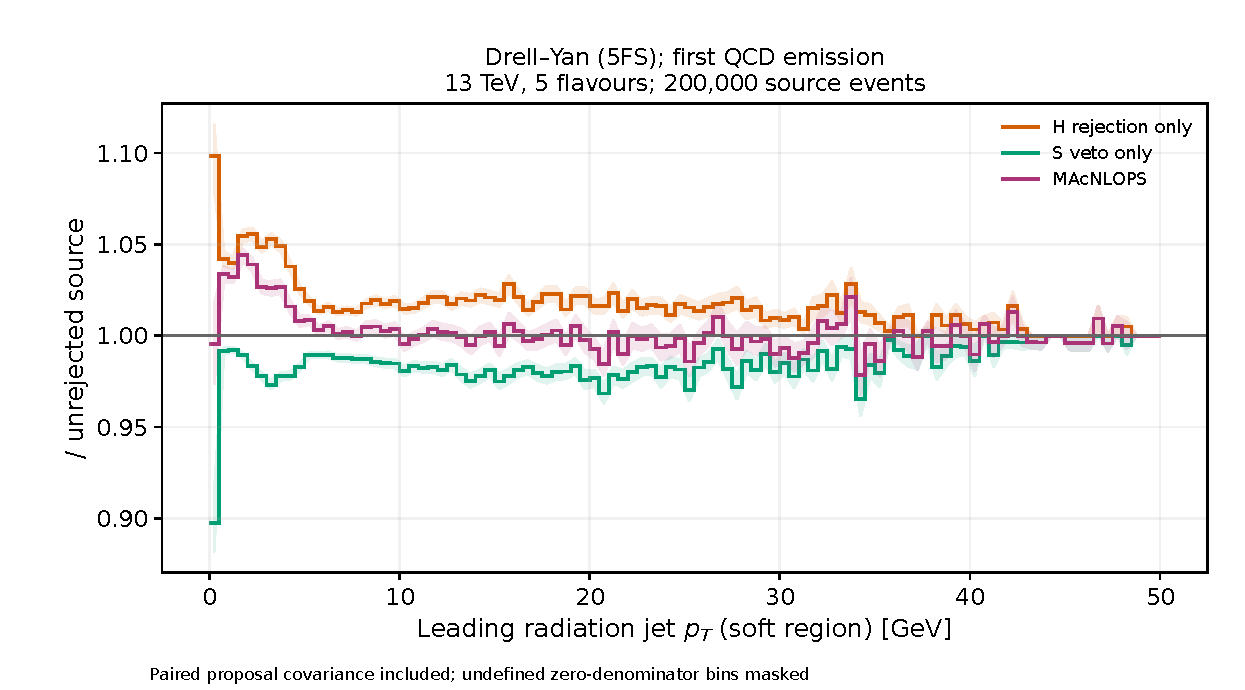
\includegraphics[width=\linewidth]{dy_first_mechanisms}
  \caption{First accepted QCD emission, with original real $H$ endpoints.}
 \end{subfigure}
 \par\medskip
 \begin{subfigure}{0.98\textwidth}
  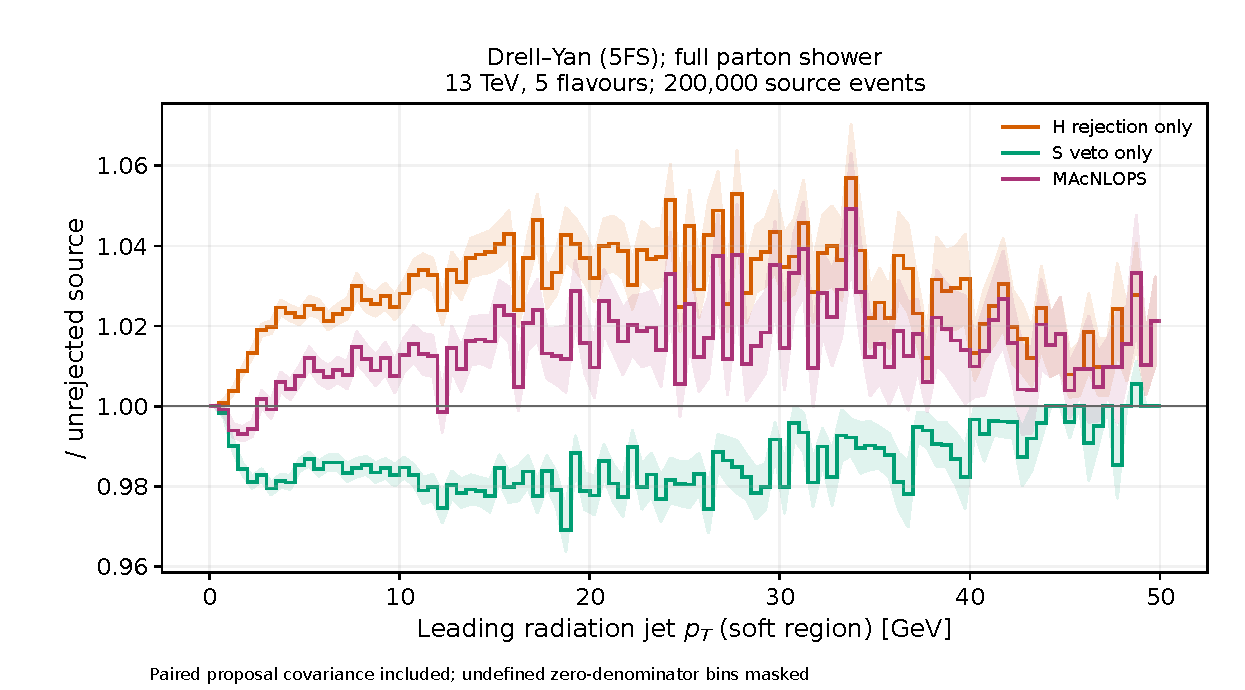
\includegraphics[width=\linewidth]{dy_full_mechanisms}
  \caption{Full QCD shower with the same original-event rejection mask.}
 \end{subfigure}
 \caption{DY leading radiation-jet transverse momentum in the soft
 region. All curves are ratios to the common unrejected ordinary
 \mcatnlo{} source evolved to the indicated stage. Orange applies
 only bounded negative-$H$ removal, green only the $S$ veto, and
 magenta both. Their competition is most visible at low $\pt$.
 Bands include the paired reference covariance. A ratio close to one
 in a visible range does not establish inclusive equality. The first
 bin includes no-radiation endpoints, and out-of-range tails are not
 shown.}
 \label{fig:dy}
\end{figure}

Figure~\ref{fig:dy} separates the two changes at first emission and
after full showering. The partial cancellation is visible, together
with a remaining change in the lowest bins. No independent sample
normalization has been applied. Full-shower smearing changes where
events populate the jet observable but does not change the inclusive
accounting in Table~\ref{tab:rates}.

\subsection{Remaining negative hard events}
\label{sec:negativeh}
\begin{table}[t]
\centering\small
\setlength{\tabcolsep}{5pt}
\begin{tabular}{lrrrrrr}
\toprule
Process & Input $H^-$ & $K_g=0$ & $H_-/K_g>1$ & Max. ratio & Kept $H^-$ & Kept weight [pb]\\
\midrule
DY & 4168 & 24 & 1 & 1.8851 & 25 & -0.28434983\\
$ZZ$ & 2511 & 10 & 1 & 1.3472 & 10 & -0.00080624\\
$t\bar t$ & 28714 & 9 & 12 & 3.4281 & 13 & -0.07558305\\
$W^+b\bar b$ & 13392 & 0 & 22 & 5.5797 & 6 & -0.02090369\\
\bottomrule
\end{tabular}
\caption{Required and realized negative-hard residuals. The zero-kernel and finite-overshoot columns count source points requiring nonzero survival probability (79 in total). The maximum excludes zero-denominator points. The kept count (54 in total) is one Bernoulli realization.}
\label{tab:residuals}
\end{table}

Table~\ref{tab:residuals} distinguishes source points with a nonzero
required survival probability from the number that actually survive
the Bernoulli draw. A finite $H_-/K_g>1$ leaves a fractional residual;
when $K_g=0$ the negative event must be kept. The numbers demonstrate
strong suppression of negative $H$, but not exact removal.

Saved native decompositions of all 79 exceptional source points
identify several concrete mechanisms:
\begin{itemize}
 \item In DY, all exceptional points project onto bottom-initiated
 Born channels. Twenty-four have $K_g=0$ because the contributing
 histories fail the heavy-threshold/$z$ support or the eligibility
 boundary. The remaining point has $H_-/K_g=1.8851$: one important
 hard-counterterm history lies below the heavy matching boundary,
 leaving too small an eligible denominator.
 \item In $ZZ$, ten points have zero eligible support. The one finite
 excess is a light $u\bar u\to ZZg$ point above the light cutoff,
 with $H_-/K_g=1.3472$. Its additive soft G completion makes the
 ordinary counterterm larger than the scalar density; this example
 cannot be explained by a heavy-quark threshold.
 \item In $t\bar t$, nine points have $K_g=0$ and twelve have a finite
 excess, reaching $3.4281$. ISR eligibility restrictions and the
 post-rescaling massive-top FSR cutoff both remove available scalar
 support. The source includes both Born-colour flows. Spin terms in
 these exceptional points are too small to explain their large
 ratios.
 \item In $Wb\bar b$, all 22 exceptional points have positive $K_g$,
 but $H_-/K_g$ reaches $5.5797$. At the largest point a bottom-FSR
 history has $q_{\rm MC}=9.0682\GeV$, above its local corrected
 colour-dipole upper scale $7.8378\GeV$. Its raw scalar contribution
 vanishes while the ordinary soft G replacement remains. Fifteen
 of the 22 points contain this type of history.
\end{itemize}
These are statements about inspected exceptional points, not an
integrated causal decomposition of the complete rate shifts. Removing
G terms only in the evaluator would not fix the ordinary-input method:
it would evaluate a different hard density from the one that generated
the source.

Negative $S$ events also remain. The retained negative-$S$ counts are
9,947 (DY), 9,130 ($ZZ$), 10,750 ($t\bar t$) and 17,509 ($Wb\bar b$).
They arise from the signed ordinary $S$ coefficient and are not cured
by a nonnegative acceptance. Even complete negative-$H$ cancellation
would therefore not make these particular samples positive weighted.

\subsection{Coloured final states and a colour-singlet control}
\begin{figure}[p]
 \centering
 \begin{subfigure}{0.98\textwidth}
  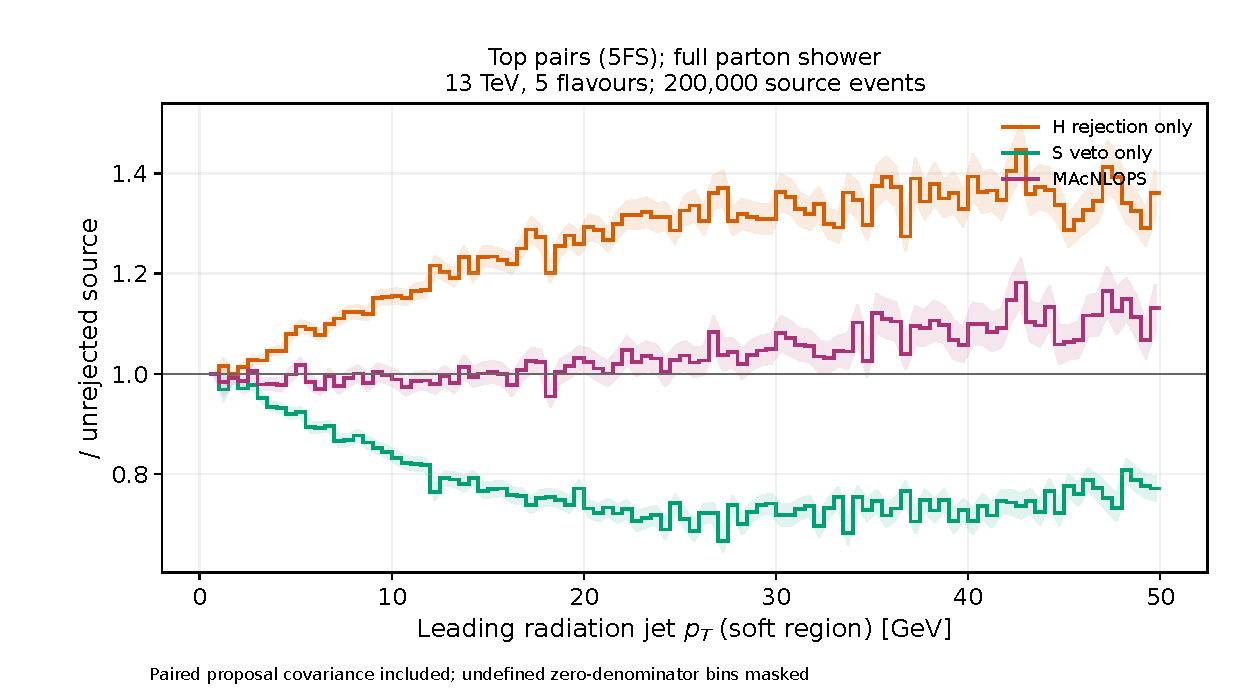
\includegraphics[width=\linewidth]{ttbar_full_mechanisms}
  \caption{Separate removal and veto ratios after full showering.}
 \end{subfigure}
 \par\medskip
 \begin{subfigure}{0.98\textwidth}
  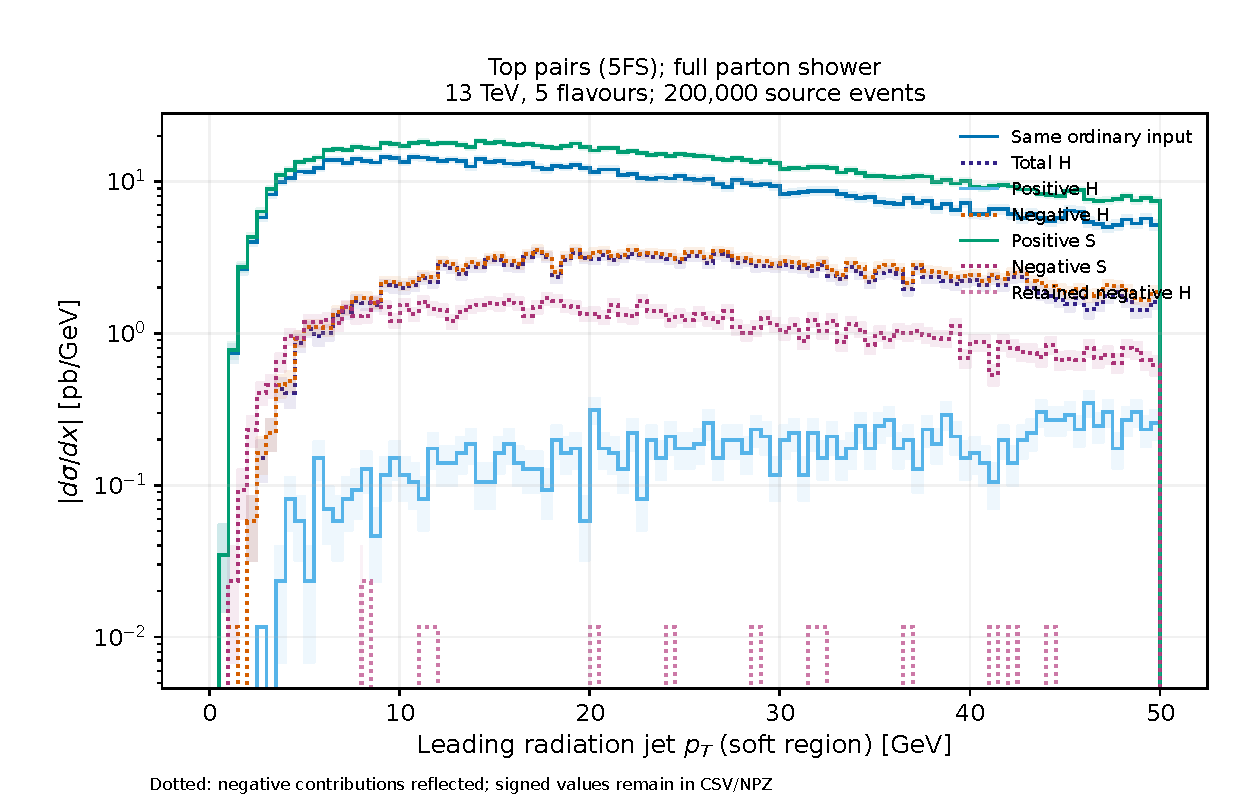
\includegraphics[width=\linewidth]{ttbar_full_source_signs}
  \caption{Signed-source decomposition, with negative curves reflected.}
 \end{subfigure}
 \caption{Top-pair leading radiation-jet transverse momentum. The
 upper panel shows the strong competition of hard removal and soft
 veto relative to the common reference. The lower panel shows
 magnitudes of signed source contributions on a logarithmic scale;
 dotted negative contributions must be subtracted, not added.
 The sparse retained negative-$H$ curve is the bounded residual.
 Top quarks are stable and excluded from radiation jets. These plots
 illustrate a sizeable finite-shower effect, not exact rate recovery.}
 \label{fig:tt}
\end{figure}

The $t\bar t$ sample has 28,714 negative $H$ source records, exceeding
its 13,112 positive $H$ records. Removing nearly all of those negative
weights therefore produces a large gain, $166.8699\pb$. The signed
$S$ loss, $123.3632\pb$, does not compensate it. Figure~\ref{fig:tt}
shows both the finite-shower effect and why a signed decomposition is
more informative than a plot containing only the final total. The
small required negative-hard remainder is not the origin of the
$43.5068\pb$ excess.

\begin{figure}[p]
 \centering
 \begin{subfigure}{0.90\textwidth}
  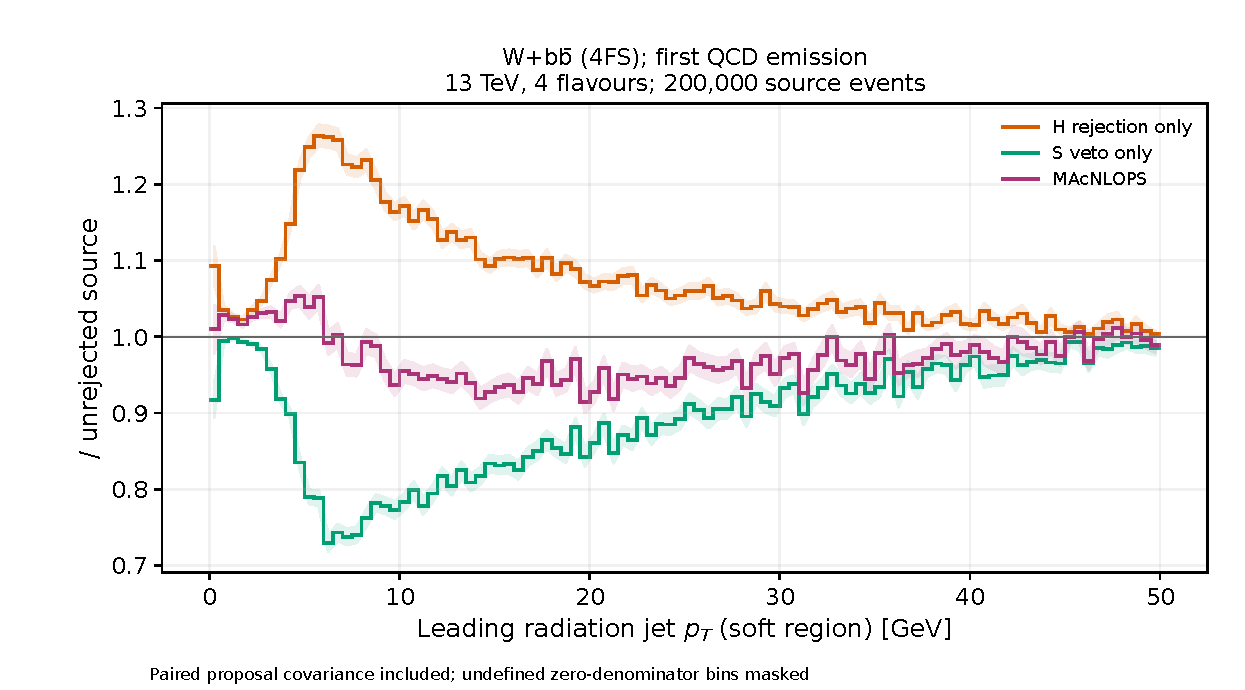
\includegraphics[width=\linewidth]{wbb_first_mechanisms}
  \caption{First-stage soft radiation-jet mechanism ratios.}
 \end{subfigure}
 \par\medskip
 \begin{subfigure}{0.90\textwidth}
  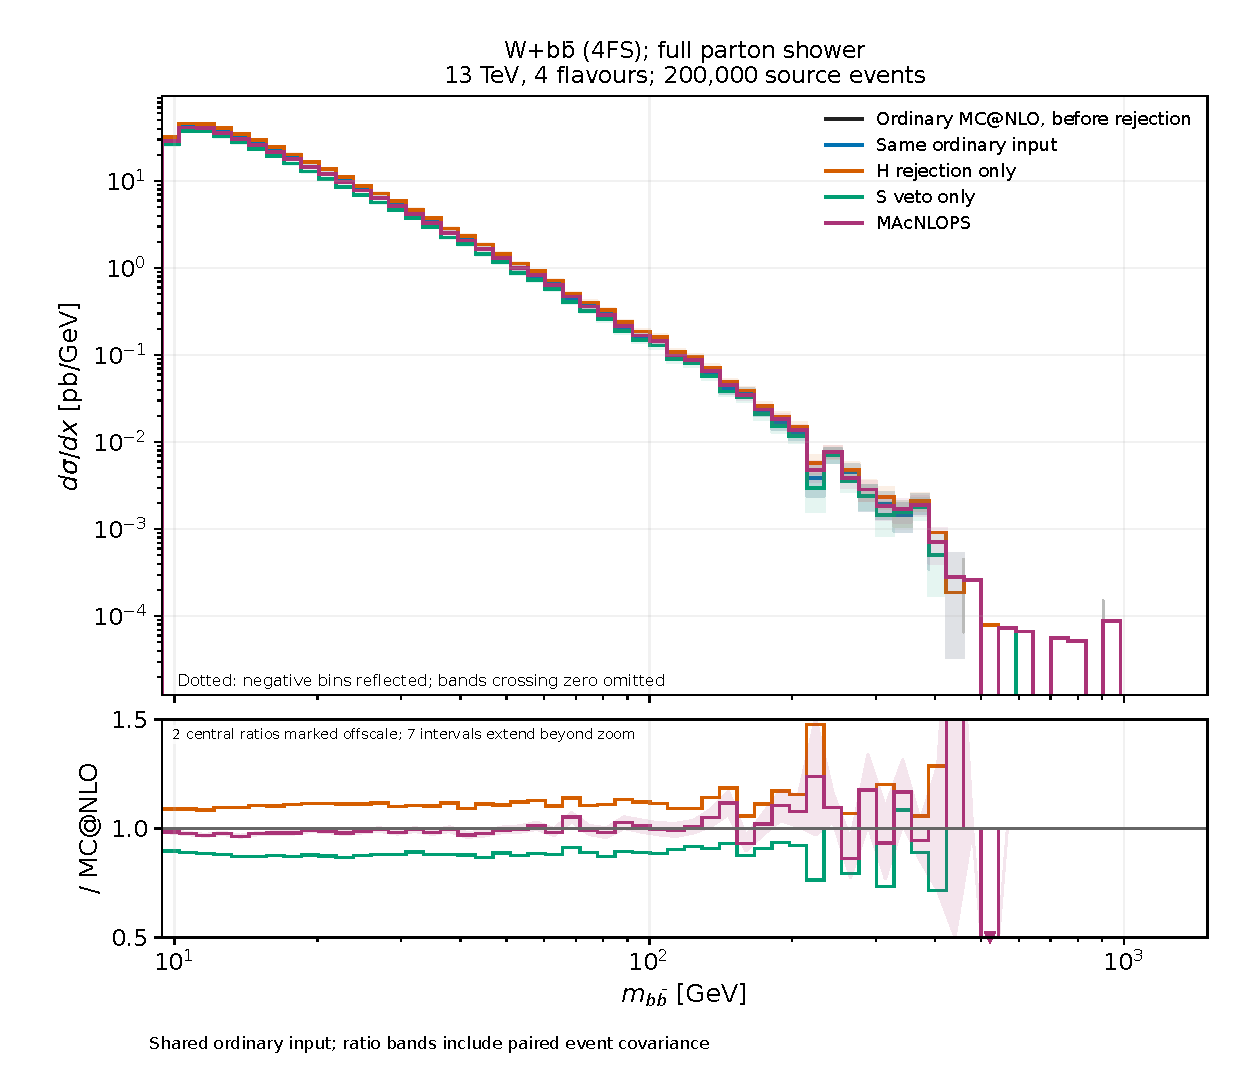
\includegraphics[width=\linewidth]{wbb_full_pair_mass}
  \caption{Full-shower bottom-pair mass and treatment/reference ratio.}
 \end{subfigure}
 \caption{Four-flavour $W^+b\bar b$ with $m_b=4.7\GeV$. The first
 panel isolates the two rejection operations. The second examines a
 hard-system observable after QCD evolution, using the selected
 bottom and antibottom rather than a reconstructed hadronic object.
 Its logarithmic mass axis resolves the populated region above
 $2m_b=9.4\GeV$. The panels do not themselves isolate G-function
 effects; those are established by the native density decompositions.}
 \label{fig:wbb}
\end{figure}

For $Wb\bar b$, $S$ rejection is stronger than the hard-removal gain
in signed rate. Figure~\ref{fig:wbb} includes both a radiation-sensitive
first endpoint and the bottom-pair invariant mass after full showering.
Keeping a genuinely four-flavour PDF/coupling/splitting profile and
massive bottom kinematics is essential to interpreting this example;
it is not a massless five-flavour proxy.

\begin{figure}[t]
 \centering
 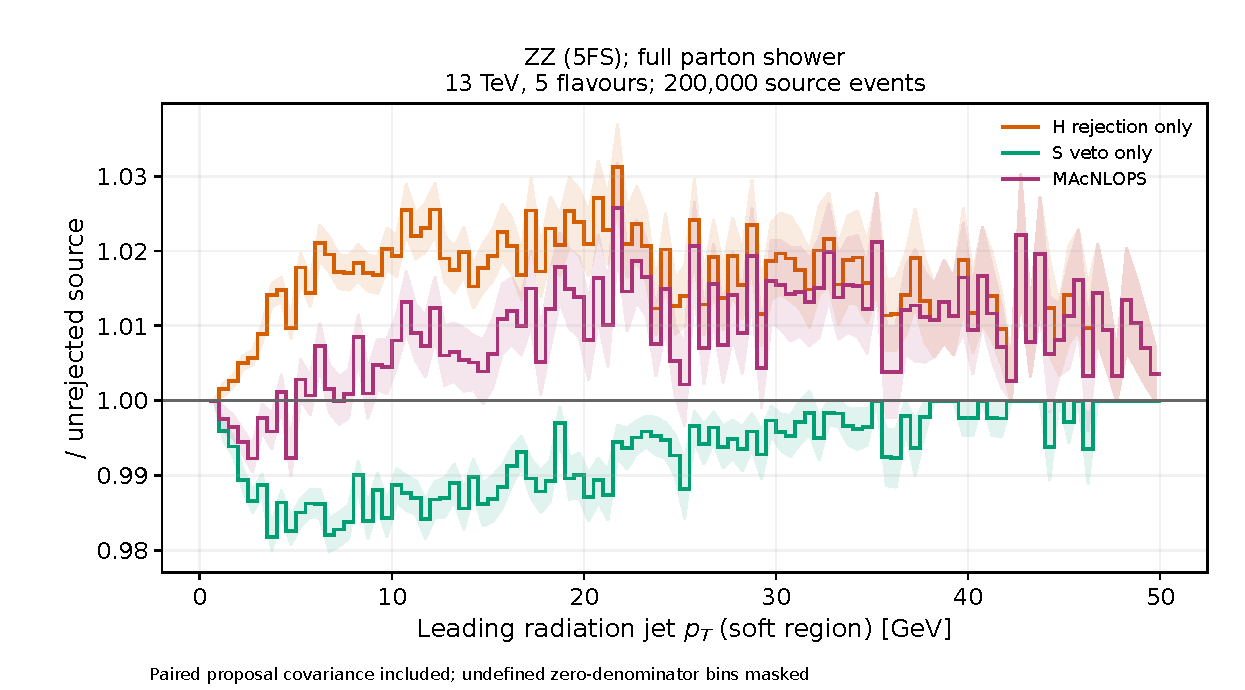
\includegraphics[width=0.98\textwidth]{zz_full_mechanisms}
 \caption{Stable $ZZ$ control after full QCD showering. The definitions
 and paired-ratio conventions are those of Fig.~\ref{fig:dy}.
 The inclusive change is comparatively small but nonzero. This
 control does not remove the counterterm/support issue: one finite
 light-flavour G-completion exception remains in the source
 classification of Table~\ref{tab:residuals}.}
 \label{fig:zz}
\end{figure}
The stable $ZZ$ result in Fig.~\ref{fig:zz} provides a colour-singlet
control without external lepton-recoil presentation. Its relatively
small integrated shift does not supply a general theorem of exact
compensation. Together, the four processes show that the finite
difference is process dependent in both size and sign.

\FloatBarrier
\section{Validation scope and limitations}
\label{sec:validation}
The manuscript's equations, source definitions and quoted numbers were
checked against the source/runtime version frozen for this calculation
and its saved production records.
All 800,000 source events have completed integrity, hard-point,
configuration and signed-accounting checks; all 172,047 source $H$
records passed the density/sign gate. Independent native configuration
checks completed for all four full-shower productions. Targeted tests
also cover inverse ISR/FSR maps, phase-space factors, support, mass-shell
guards, source partitioning, hard annotations and the corrected
matrix-element evaluation.

An independent particle-level check completed for the first 5,000
original events of each process, covering 40,000 raw first/full
endpoints and the corresponding retained events, including forced
heavy conversions. The remaining whole-production particle audit and
the final independent histogram/package audit were deliberately
stopped or skipped. Earlier complete-process histogram reviews exist
for DY, $ZZ$ and $Wb\bar b$; the analogous final $t\bar t$ review was
not completed. Accordingly, this paper does not claim an exhaustive
independent particle-level certificate for all 800,000 events. The
reported complete accounting and configuration evidence is distinct
from that unfinished check.

Several physical limitations remain. The implementation is not a
generic importer of arbitrary existing remassed LHE records. Some
massive pair/sister inverse maps are outside its declared first-step
scope. Negative $S$ weights remain, and source G/support differences
require signed $H$ residuals. The observed finite changes are not
covered by a proof of exact all-order normalization or universal
logarithmic equivalence. A numerical distribution difference alone
also does not establish whether its size lies within a particular
perturbative uncertainty band; such an uncertainty study was not
performed here.

\section{Discussion and conclusions}
\label{sec:conclusion}
An ordinary \mcatnlo{} source can be used for the removal/veto idea
without changing its G completion, bogus factor or integrated source
compensation, provided its actual signed partition and hard momenta
are available. The reference and pre-veto treatment then coincide
exactly because they are views of one cohort. The hard-momentum
annotation and aligned shower masses make the required density
evaluation well defined while leaving the ordinary event-body writer
available.

Complete negative-hard removal, however, is not always compatible
with a bounded veto using the available scalar shower density. The
bounded common-source construction used here keeps $H_--\min(H_-,K_g)$ with its
negative sign. Heavy-threshold gates, massive-FSR cutoffs, dead zones
and additive G completions explain the observed exceptional points.
Simply adding the bogus factor or clipping a probability cannot
remove that requirement.

The remaining distribution difference has a separate, more general
origin: the signed, evolved first-emission $S$ density is not the
leading denominator. Equation~\eqref{eq:exactdifference} identifies
the precise inclusive mismatch, and Eq.~\eqref{eq:fulloperator}
extends it to subsequent showers. The corrected spinor evaluation
removes a numerical defect; it does not make those finite expressions
identical. The $t\bar t$ result especially calls for treating the
remaining finite prescription dependence as a substantive numerical
effect rather than assuming near-exact compensation.

Exact finite-coupling cancellation would require a compatible
conditional construction using the actual evolved density, as well
as positivity and support. That density is signed in the present
source, so merely replacing $K_g$ by an estimated finite-shower
histogram is not a general acceptance algorithm. An alternative
resolved source can make the leading bound automatic, but changes
the starting sample and its integrated $S$ compensation. These are
distinct possible developments. The current results support a
carefully bounded, strongly negative-$H$-reducing method with explicit
residuals and finite-shower differences; they do not support a claim
of universally positive events or exact \mcatnlo{} reproduction after
the removal and veto.

\appendix
\section{Ordinary and resolved source modes}
The implementation contains an optional resolved-source path, which
is \emph{not} used for the results above. With the same eligibility
indicator its schematic densities are
\begin{equation}
 D_h^*=(1-g_h)R_h+g_hK_{0,h},\qquad
 H^*=\sum_hg_h(R_h-K_{0,h}).
 \label{eq:legacy}
\end{equation}
For nonnegative $R_h$, $\pos{-H^*}\le\sum_hg_hK_{0,h}$, so the leading
bound follows. But $D^*$ must also replace the integrated counterterm
in $S$. It changes the source's low-scale support and G treatment.
Adding a damping factor to that source does not turn it into the
ordinary source of Eq.~\eqref{eq:hord}. The reported common production
sets \code{macnlops\_resolved\_source=False}; the workflow option
\code{macnlops=True} alone does not select Eq.~\eqref{eq:legacy}.

\section{Reproducibility and data provenance}
\label{app:repro}
The source collection is labelled \code{common\_200k\_v2}. Source seeds
are 20261101--20261104 in process order DY, $ZZ$, $t\bar t$, $Wb\bar b$.
They are taken from the frozen generation records, not mutable current
run cards. The local production root is
\code{/export/tmp/rikkert/macnlops\_common\_20261020}.
The companion source package contains a machine-readable evidence
manifest with the source, accounting and figure checksums; it does
not duplicate the large event samples.

The rate table comes from \code{analysis/final\_accounting\_review.json}
and its complete signed-statistics report. Exceptional-point counts
and mechanisms come from the two
\code{analysis/required\_residual\_diagnostics*.json} reports and their
native history decompositions. The selected vector plots are unchanged
copies from the final \code{plots/} collection. The full collection
has 72 pages; seven panels are selected here. Original source and
accepted weights, no-emission endpoints and histogram flow bins are
retained in the underlying records.

Useful code entry points are \code{fks\_singular.f} and
\code{montecarlocounter.f} for the ordinary source;
\code{add\_write\_info.f} and \code{handling\_lhe\_events.f} for hard-point
capture and annotation preservation;
\code{driver\_macnlops.f} and \code{mc\_pythia8\_kernel.f90} for native
history/density evaluation; \code{native\_histories.py} for exported
matrix-element evaluation; \code{MacNLOPS.cc} for first-emission endpoints; and
\code{madgraph/various/macnlops.py} for preparation and rejection.
The full-shower figures used the now-retired native validation driver;
its archived source identity remains in the evidence manifest.
The frozen certified proposal used source copies named
\code{MacNLOPSPDFBounds.cc} and
\code{prepare\_macnlops\_pdf\_envelope\_patch.py}, identified in the
external production archives. These removed extensions are historical
implementation artifacts, not active dependencies or stock build instructions.
The companion README specifies the source directory, build command
and scope of the manuscript cross-checks.

\begingroup
\small
\setlength{\bibsep}{4pt}
\bibliographystyle{unsrtnat}
\bibliography{references,method_references}
\endgroup
\end{document}
